%! Author = adnansiddiquei
%! Date = 29/06/2024

% Preamble
\documentclass[a4paper,11pt]{article}
\pdfoutput=1

% Packages
%\usepackage[colorlinks=true, linkcolor=blue, urlcolor=blue, citecolor=blue, pdfborder={0 0 0}]{hyperref}
\usepackage{url}
\usepackage{jcappub}
\usepackage[T1]{fontenc}
\usepackage{listings}
\usepackage{roboto}
\usepackage{subcaption}
\usepackage{blindtext}
\usepackage{seqsplit}
\usepackage[nottoc]{tocbibind}
\usepackage{siunitx}
\DeclareSIUnit\angstrom{\text {Å}}

%\newcommand{\inlinecode}[1]{\lstinline{#1}}
%\newcommand{\inlinecode}[1]{\texttt{#1}}
\newcommand{\inlinecode}[1]{\texttt{\seqsplit{#1}}}
\lstset{basicstyle=\fontfamily{pcr}\selectfont}


\title{\boldmath Reproducing AstroCLIP: Executive Summary}

% %simple case: 2 authors, same institution
\author{Adnan Siddiquei}
\affiliation{University of Cambridge}

% e-mail addresses: one for each author, in the same order as the authors
\emailAdd{as3438@cam.ac.uk}
\note{Word Count: 973 (text); 219 (figure captions).}


\begin{document}
%    \abstract{}

\maketitle
\flushbottom

\section{Background and Motivation}\label{sec:introduction}
Scientific datasets, especially in astronomy, have been expanding rapidly for decades.
Spectroscopic surveys like the Sloan Digital Sky Survey (SDSS)\footnote{https://www.sdss.org/}~\citep{york2000} and the
Dark Energy Spectroscopic Instrument (DESI)\footnote{https://www.desi.lbl.gov/} have been collating millions of galaxy spectra.
Similarly, photometric surveys like the DESI Legacy Survey~\citep{desilegacy2018} have imaged vast areas of the sky,
extracting millions of sources.
A spectrum is a plot of light intensity versus wavelength, and a photometric image combines light from various filters,
as illustrated in Figures~\eqref{fig:example-spectra} and ~\eqref{fig:bandpass-illustration}.

Both photometric and spectroscopic surveys are essential tools in modern astronomy and these datasets are used for
a variety of scientific purposes, from understanding the large scale structure of the universe;
estimating galaxy properties such as redshift, stellar mass, and star formation rate; to identifying rare objects such as
quasars and supernovae; and many more.
However, the growing data set size and diversity makes much of this difficult and traditional methods are often
limited by the quality of the data and its associated labels.
One such example is morphological classification, where we desire to classify galaxies into different types based on their
shape and structure, such as spiral or elliptical.
A decade ago we had crowdsourced campaigns such as Galaxy Zoo 2~\citep{willet2013} which classified approximately
300,000 galaxies, we now have tools such as Tractor\footnote{https://github.com/dstndstn/tractor}
which can probabilistically identify sources from photometric surveys and infer properties such as morphological classification.
More recently, given the unavailability of high quality labels, unsupervised and self-supervised learning methods have been
gaining popularity to tackle these sorts of tasks.
For example:
\begin{itemize}
    \item \cite{liang2023} train a 1D convolutional spectrum autoencoder on spectral data for the purposes of outlier
    detection;
    \item \cite{stein2021} train a 2D convolutional image embedder using a self-supervised technique on galaxy images
    for the purposes of similarity search;
    \item \cite{hayat2021} also use a self-supervised technique to train a 2D convolutional model to estimate distances to galaxies from their
    photometric images, and further demonstrate that the learned embeddings can be fine-tuned very effectively for redshift estimation;
\end{itemize}
\cite{hayat2021} also show that significantly better performance can be acquired through fine-tuning the self-supervised
pre-trained model compared to simply training a supervised model from scratch.
This conclusion is not uncommon in the field of machine learning outside of astronomy and demonstrates the power
of transfer learning and the importance of foundation models for astronomical datasets.

However, as of yet most of these self-supervised learning methods have only been applied to a single modality despite
promising results in cross-modal contrastive learning outside of astronomy, such as contrastive language-image pre-training CLIP~\citep{radford2021}.
~\cite{astroclip} pioneer on this front by proposing a multi-modal contrastive learning approach to embed galaxy spectra
and galaxy images into a shared low-dimensional latent space, and in this paper we reproduce their results.
Given the multi-modal nature of astronomical datasets, a useful astronomical foundation model should be able to embed
the varying views of the same object effectively into a shared latent space, allowing for in-modal and cross-modal downstream
application through zero-shot or few-shot learning.

\begin{figure}[t]
    \centering
    \makebox[\textwidth]{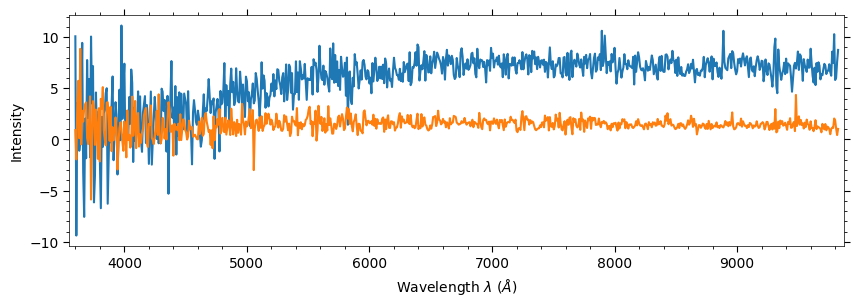
\includegraphics[width=1\textwidth]{figures/example_spectra}}
    \caption{An example of two galaxy spectra.}
    \label{fig:example-spectra}
\end{figure}
\begin{figure}[t]
    \centering
    \makebox[\textwidth]{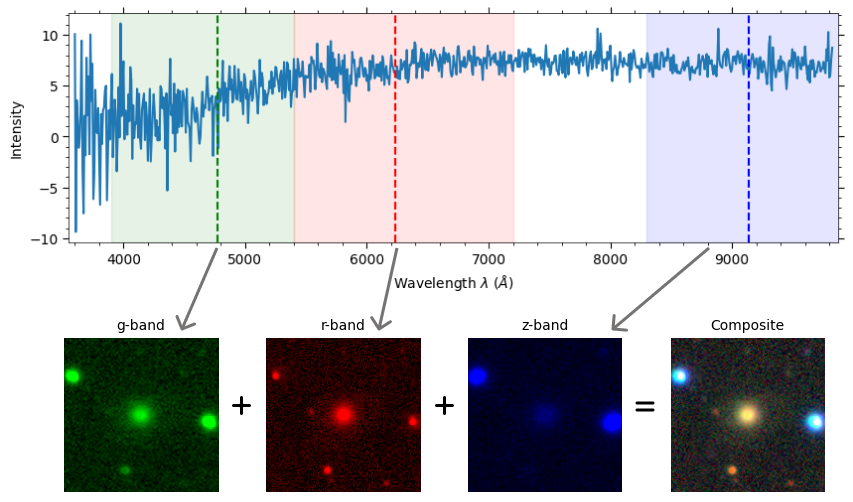
\includegraphics[width=1\textwidth]{figures/bandpass_illustration}}
    \caption{Bandpasses for various filters, illustrating how they combine to form a photometric image.
    The dotted line indicates peak transmission wavelengths; the shaded areas show the transmission range.
    This Figure is a conceptual illustration, and not exact.}
    \label{fig:bandpass-illustration}
\end{figure}

\section{A Review of AstroCLIP}\label{sec:original-paper}
\cite{astroclip} present AstroCLIP, a cross-modal foundation model for galaxies.
The approach involves two components.
Initially, they pre-trained a transformer-based spectrum embedder on spectroscopic data from the DESI Early Data
Release~\citep{desiearly2023} using a self-supervised technique.
They also pre-trained a vision transformer for images from the DESI Legacy Survey~\citep{desilegacy2018} using the DINO
v2 framework~\citep{oquab2024}.
Secondly, they fine-tuned both embedders under the InfoNCE loss~\citep{oord2019} to align embeddings in a 512-dimensional
latent space.
The InfoNCE loss promotes proximity in embeddings of the same object and distance for different objects,
where proximity is measured through the cosine similarity (or equivalently, the normalised dot product)
of the embeddings.

They demonstrate that the embeddings are well-aligned by using the embeddings to perform a variety of downstream zero-shot
and few-shot tasks, including in-modal and cross-modal similarity search, redshift prediction, and galaxy property prediction.
The model was never explicitly trained to embed these properties into the latent space, but these properties inherently
exist in the data and as such, well-aligned embeddings should be able to make effective zero-shot and few-shot predictions
on these properties.

\section{Reproduction}\label{sec:reproduction}
\begin{figure}[t]
    \centering
    \makebox[\textwidth]{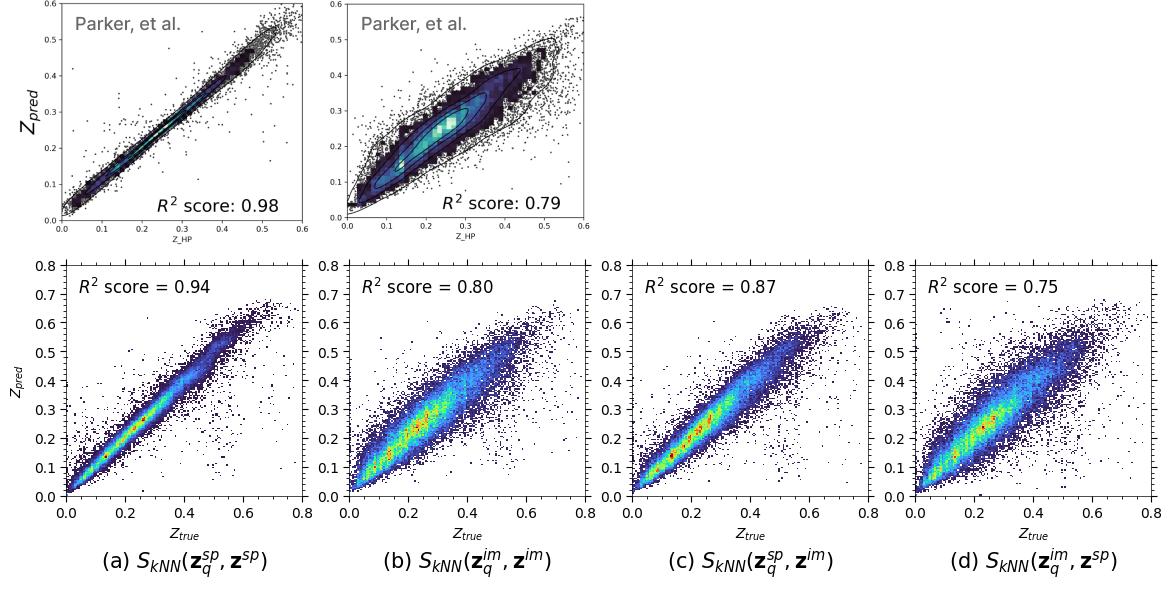
\includegraphics[width=1\textwidth]{figures/redshift_knn_regression_parker}}
    \caption{k-NN regression for zero-shot redshift prediction, showing predicted vs. true redshift.
    Top row is results from \cite{astroclip} for their 512-dim embedding model, bottom row is results from our 128-dim embedding
    model.
    $S_{kNN}(\mathbf{z}_{q}^{sp}, \mathbf{z}^{im})$ indicates the cross-modal prediction type where a spectrums redshift was
    predicted using its 16 closest embeddings derived from galaxy images.}
    \label{fig:rkr}
\end{figure}

\begin{figure}[t]
    \centering
    \makebox[\textwidth]{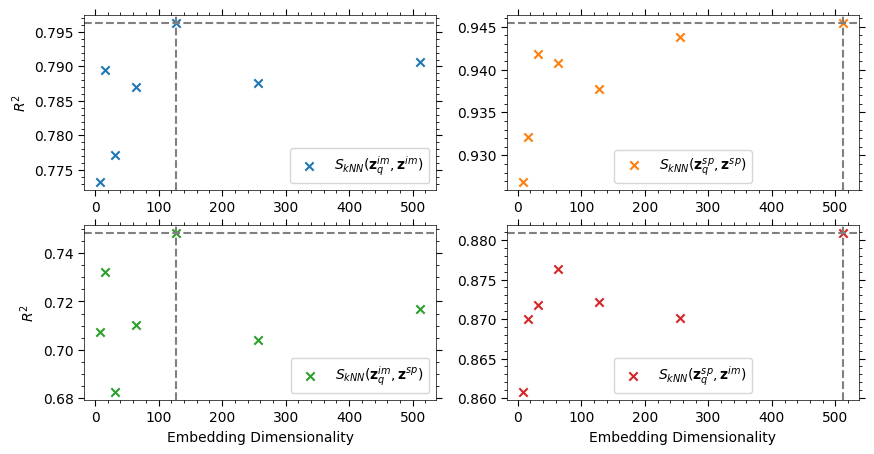
\includegraphics[width=1\textwidth]{figures/r2_vs_embedding_dim}}
    \caption{Consolidated results for all embedding dimensions and prediction types, displaying $R^{2}$ values vs. embedding dimensionality.
    These are the $R^{2}$ values derived if Figure~\eqref{fig:rkr} were plotted for all embedding dimensionalities.}
    \label{fig:r2_vs_embedding_dim}
\end{figure}

\begin{figure}[t]
    \centering
    \makebox[\textwidth]{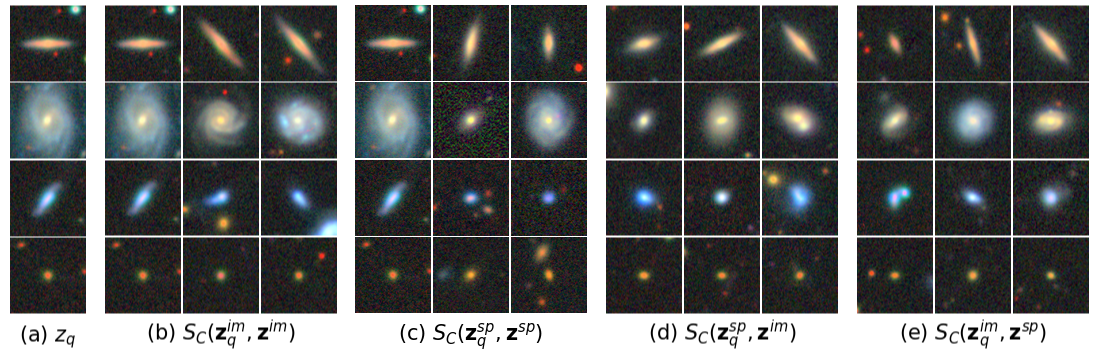
\includegraphics[width=1\textwidth]{figures/sim_search_images_all}}
    \caption{Cosine similarity search results using the 128-dimensional model. (a) 4 Query galaxies;
        (b, c, d, e) Top 3 similar galaxies across the 4 prediction types.
        By construction, the most similar in-modal galaxy to any given galaxy is itself, hence, the first column of images
        in (b) and (c) are identical to the query image in (a).}
    \label{fig:ssia}
\end{figure}

\begin{figure}[t]
    \centering
    \makebox[\textwidth]{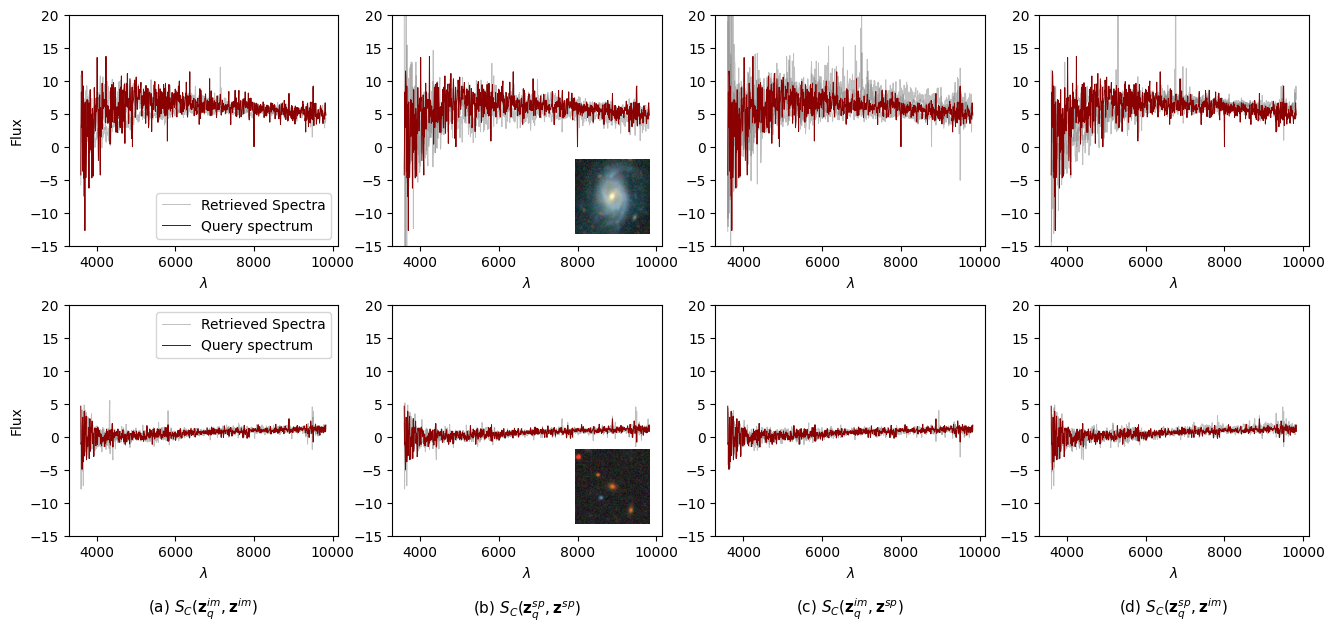
\includegraphics[width=1\textwidth]{figures/sim_search_spectra}}
    \caption{Cosine similarity search for spectra using the 128-dimensional model.
    Each row shows a query galaxy (galaxy imaged in (b)), each subfigure shows the 3 most similar spectra to the query galaxy
       for the given prediction type.}
    \label{fig:sss}
\end{figure}

We reproduce the AstroCLIP model, however we utilise the pre-trained convolutional spectrum embedder by ~\cite{liang2023}
and the pre-trained convolutional image embedder by ~\cite{stein2021} rather than pre-training our own.
We use the dataset as provided by ~\cite{astroclip}, and a variety of general and astronomy specific data augmentations
to increase the variety of the dataset.
In addition to the 512-dimensional model, we also train AstroCLIP variations to embed the spectra and images into
a variety of lower-dimensional latent spaces: $[8, 16, 32, 64, 128, 256]$.
We train each of these 7 models for 75 epochs, and choose the model with the lowest validation loss for analysis.

We assess the performance of our models using a subset of the downstream tasks presented in the original paper, specifically
zero-shot k-NN redshift estimation and retrieval by cosine similarity, these results are displayed in Figures~\eqref{fig:rkr},
~\eqref{fig:r2_vs_embedding_dim}, ~\eqref{fig:ssia}, and ~\eqref{fig:sss}.
Generally, we find equivalent performance in our reproduction.
As shown in Figures~\eqref{fig:rkr}, we outperform their 512-dimensional model in the photometric redshift prediction task
(across a larger redshift range) with our 128-dimensional model, achieving an $R^{2}$ value of 0.80 compared to their 0.79; but
fall short in the spectroscopic redshift prediction task with an $R^{2}$ value of 0.94 compared to their 0.98.
We also show that model performance stays generally stable with embedding dimensionality as low as 8, as shown in
Figure~\eqref{fig:r2_vs_embedding_dim}.
Cosine retrieval results are also consistent with the original paper, as shown in Figures~\eqref{fig:ssia} and ~\eqref{fig:sss}.

\section{Significance of Results}\label{sec:conclusion}
Our results, alongside those of~\cite{astroclip}, demonstrate that it is possible to achieve high quality foundation
models for astronomical data using cross-modal contrastive pre-training, and that the learned embeddings can be used for a variety
of downstream tasks with strong performance.
This has a variety of impacts on the field of astronomy, such as enabling cross-modal similarity searches for rare or interesting
objects, and enabling the use of pre-trained foundation models for transfer learning on smaller datasets for specific tasks,
thereby reducing the requirement for large amounts of high quality labels.


\clearpage

%\nocite{*}
\bibliographystyle{apalike}
\bibliography{exec-summary}
\clearpage

%\appendix

%\section{Appendix A}\label{app:app-a}
%Lorem ipsum dolor sit amet, consectetur adipiscing elit. Suspendisse eget urna laoreet, elementum tellus nec, dapibus dui.
\end{document}
